
\section{RESULTS}
\label{sec:results}

We obtained data for each parameter of interest by running the simulation for
ten trials, recording the value for each student for every year of the
simulation. Often, this was the proportion of that individual's friends who
are minorities, but on occasion we were interested in other variables. We
considered only the value corresponding to each student's senior year. Also,
when considering friendship proportions, we omitted the data for students who
had zero total friends. 

For analysis, we formed two vectors (arrays) of the values of interest, one
for white students and one for minority students, concatenating all students
of that race from across all trials. The resultant vectors were around 160,000
in length for the white data and around 40,000 in length for the minority
data.

To compare the populations, we chose to use the Wilcoxon rank test (as opposed
to the more common Student's t-test) because much of our data is decidedly
non-normal. Figure 1 illustrates this fact by using the proportion of minority
friendships data as an example. A histogram of all values for one set of ten
trials (both white and minority data included) is most closely modeled by the
beta distribution instead of a normal distribution. (A Q-Q plot, not shown,
gave evidence of non-normality). We use the standard $\alpha=0.05$ rejection
value for $p$.

\begin{figure}[ht]
  \centering
    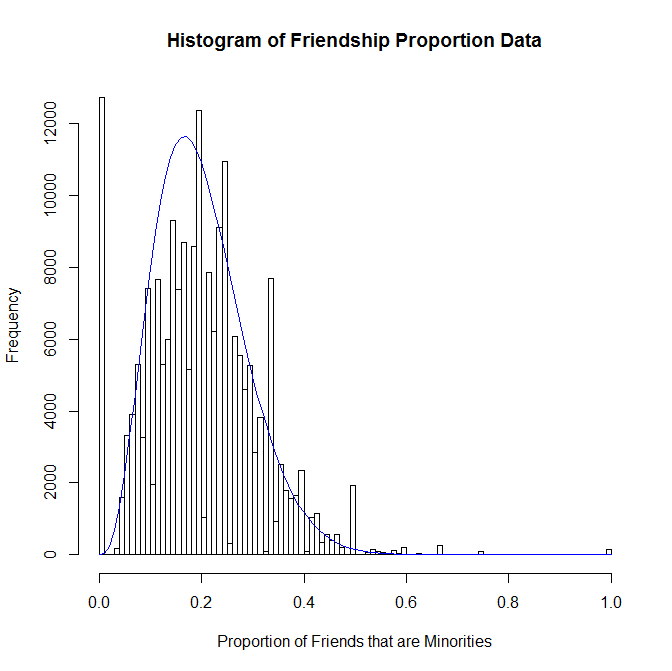
\includegraphics[width=0.5\textwidth]{histogramProportionData.png}
      \caption{A histogram of the minority friendship proportion data compared
to an ideal Beta distribution.}
\end{figure}

\subsection{Simulation Verification}

%\begin{figure}[h]
%  \centering
%    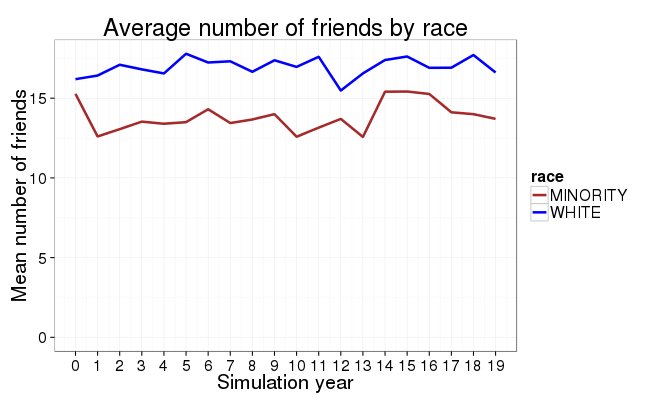
\includegraphics[width=0.5\textwidth]{avgNumberOfFriendsFromCaladan.png}
%      \caption{The average number of friends students possessed for one run of the simulation.}
%\end{figure}

We first consider the average number of friends held by minorities and whites
across all years in the simulation to verify that segregation occurs. We see 
that for any $w_r\neq 0$, minorities had fewer friends on average than whites,
regardless of other parameter settings. The following table shows the average
number of friends held by each of the two races, with the associated $p$-value
used to determine if the difference is significant.\\

\begin{table}[htb]
\centering
\caption{For varying race weights, the average number of friends that white
students and minority students have during senior
year.\label{friendshipsVsRaceWeight}}
\begin{tabular}{|c|c|c|c|}
\hline
$w_r$ & White students: mean \# of friends & Minority students: mean \# of
friends  & $p$-value\\
\hline
0 & 15.66 & 15.73 & 0.0784\\
10 & 15.54 & 14.15 & $<2.2\times 10^{-16}$\\
20 & 15.49 & 12.97 & $<2.2\times 10^{-16}$\\
100 & 15.43 & 7.90 & $<2.2\times 10^{-16}$\\
\hline
\end{tabular}
\end{table}

That is, if race matters even slightly to the students in the simulation, then
minorities will form fewer relationships. When race is not a factor in
friendship formation, the races have an approximately equal average number of
friends, as expected. Additionally, the number of friends held by whites does
not vary for varying $w_r$, indicating that $w_r$ does not directly impact
their ability to form and maintain relationships, at least for $p_w=.85$.

%%By creating stacked histograms of the racial composition of each group,
%We observed that the composition of groups at the null 
%race weight matched the expected composition, which was based on the population composition, more closely than any of the 
%nonzero race weights. As race weight increased, the observed group composition grew farther from that which was expected. In 
%fact, at the most extremely high values of race weight, an increasing proportion of the groups consisted only of white 
%students, as minorities lose affinity towards many groups, and thus can neither join nor remain in them.

%We used boxplots to track and display the frequency of perceived similarity levels whenever two students encountered each other.

For $w_r=0$, students participating in interracial encounters perceived the
same average similarity levels as students involved in same-race encounters,
as expected. For higher values of $w_r$, the homogeneous race interactions had
similarity values that remained at approximately the same level. Meanwhile,
the perceived similarity of heterogeneous race interactions creeped lower.

\begin{figure}
\begin{subfigure}{.5\textwidth}
  \centering
    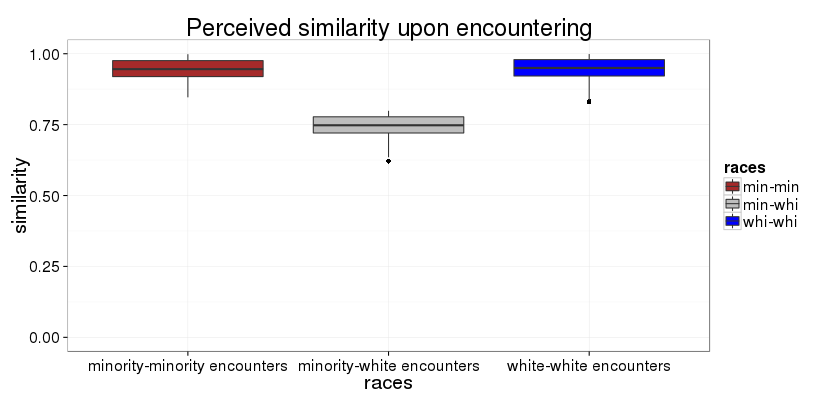
\includegraphics[width=1.2\textwidth]{similarityBoxplots20.png}
      \caption{Perceived similarity.}
\end{subfigure}
\begin{subfigure}{.5\textwidth}
    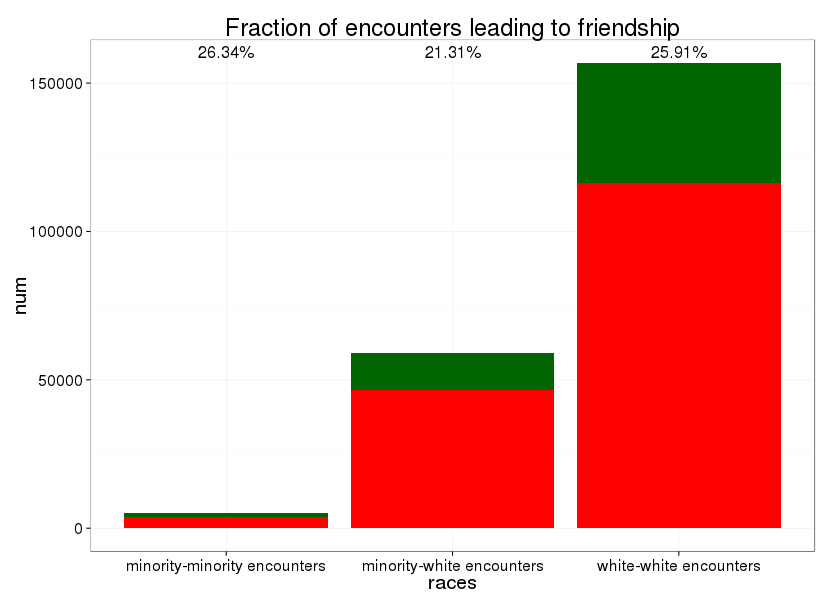
\includegraphics[width=\textwidth]{encountersGraph20.png}
      \caption{Fraction of encounters leading to friendship.}
\end{subfigure}
\caption{Perceived similarity and encounters for $w_r=20$.}
\end{figure}

Because of this, homogeneous encounters resulted in friendship slightly more
often (with respect to a percentage) than heterogeneous encounters with
$w_r>0$. As the importance of race increased, the proportion of heterogeneous
encounters which resulted in friendship decreased as expected, while the
proportion of homogeneous encounters which resulted in friendship stayed
approximately the same.

\subsection{Discoveries}

After preliminary analyses utilizing various graphs, we proceeded to analyze the data in a more concrete manner. For the following observations, we 
choose to use the proportional friendship data.

%The data generated from race weight being set to 0 was used as our baseline reference 
%for purely integrated data. So, any comparion of data to this baseline reference that was insignificant could be called integrated. The data generated 
%from race weight equalling 100 was considered to be the extremely segregated reference point. Of course, race weight is unbounded, and it would 
%be impossible to find ``the absolute" maximum race weight to case 100\% segregation. We decided that at level 100, race weight is high enough 
%to be deemed extreme segregation. So, any comparison of data to this reference point that was insignificant could be called extremely integrated.

%Some weird results from this so I won't consider it for now

First, we consider the impact of the {\bf OrientationGroups} policy. We
collected data for several values of $w_r$, both with the policy enabled and
disabled. 

We began with $n_{f_0}$ (the number of fixed-membership, intentionally
mixed-race orientation groups) set to 5, and $f_{\text{\textit{minority}}}$
(the proportion of minorities in such groups) to 0.5. For $w_r=0$, {\bf
OrientationGroups} did not demonstrate any significant effect on the
population (as measured by Wilcoxon rank test), as expected. This policy also
did not have an effect at $w_r=1$ through $w_r=10$, with the campus still as
segregated as before. When $w_r$ was increased to 20, however, the white
population did experience a significant change. Finally, for the extreme
setting of $w_r=100$, {\bf OrientationGroups} again had a significant effect
on the white data. Interestingly, with double this number of orientation
groups ($n_{f_0}=10$) the policy had a significant effect even for $w_r=1$. 

Note that since the mean is not a sufficient statistic for the beta
distribution (the information held in a distribution of this type is not
adequately captured by reporting the mean, as it would be for a normal
distribution), we do not compare or even report the means here. The
alternative hypothesis for the Wilcoxon test is not that the means are equal,
as in the Student's t-test, but instead is that the true location shift is not
zero. Therefore, two statistically significant vectors may have the same or
similar means, but come from two very different beta distributions with
differing shape parameters and location shift not equal to zero. While this
may be difficult to interpret within this context, the important conclusion is
that the policy has been verified to have a tangible effect on the
relationships formed by Students.


%The actual difference may 
%be unexpected: The policy caused the mean proportion of minority friends held by whites to \emph{decrease}, from 0.1646 to 0.1634. This is evidence that the policy actually caused higher segregation for whites. However, the positive result is that the mean proportion of minority friends held by minorities also decreased, from 0.2215 to 0.2201. This means that, on 
%average, minorities had a higher percentage of their friendships form with whites, improving the integration from their direction. 


%I left out that there was a non-significant effect on the minority data where the mean
%actually went up, so it's almost like the policy made things worse

%If a minority has fewer minority friends, they have more white friends, which means they experience more
%integration. Does that really help them at all? If I'm a minority, am I better off under a policy that causes me
%to have more white friends than I would have been otherwise? Or would it not be as much of an improvement as if I just had
%more friends in general? Or, would I feel more accepted if I could make lots of friends with people of my own race? Is the
%end game to make whites have more minority friends, or to make minorities have more white friends? Which is truly the most
%beneficial in terms of making minorities feel more accepted? Stephen?

%I could see the argument for "minorities having more friends that are white" being beneficial from the viewpoint that
%then they may not feel as threatened by other whites they encounter (may feel more at home/relaxed) as well as that the 
%spread of ideas due to interaction with people who are different is increased.

For the {\bf InitialMixedRaceDyads} policy we set $n_{d_0}$ (the number of
mixed-race friendships each Student begins with) to 10, a value which is
relatively high considering the average total number of friendships (see Table
\ref{friendshipsVsRaceWeight}). At $w_r=1$, the policy had an effect on both
races in the population. When this was repeated for $w_r=20$, the policy
appears to have had no effect. It may be that even at a relatively low value
for the importance of race, the policy is already not strong enough to
overcome the perceived barrier. We suspect that this in turn may be due to
friendship decay: even if students are initialized with mixed-race
friendships, those friendships will soon evaporate if not refreshed often
enough.
